\documentclass{article}

\usepackage{geometry}
\usepackage{mathtools}
\usepackage{graphicx}
\usepackage{subcaption}
\usepackage[hidelinks]{hyperref}
\usepackage{cleveref}
\usepackage{tikz}
\usepackage{pgfplots}


\newcommand{\mail}[1]{
  \href{mailto:#1}{#1}
}

\geometry{
  top=2cm,
  bottom=2cm,
  right=3cm,
  left=3cm
}

\pgfplotsset{
  compat=1.13,
  every axis/.prefix style={
    width=.85\textwidth,
    height=250pt,
    legend cell align=left
  },
  every axis plot/.style={
    no marks,
    line width=.8pt
  }
}

\begin{document}

\begin{center}
  \textbf{
    \LARGE Deep Learning with Stacked AEs \& RBMs \\
    \vspace{.5ex}
    \large DD2437 - Artificial Neural Networks \& Deep Architectures - Lab 4\\
    \vspace{1ex}
    \large
    \begin{tabular}{ccc}
      Niels Agerskov & Lukas Bjarre & Gabriel Carrizo \\
      \mail{agerskov@kth.se} & \mail{lbjarre@kth.se} & \mail{gabcar@kth.se}
    \end{tabular}
  } \\
  \vspace{.5ex}
  \rule{\textwidth}{0.4pt}
\end{center}

This lab will examine two different artificial neural network structures,
Auto Encodes (AE) and Restricted Boltzmann Machines (RBM).
Their effectiveness in a learning task 
and the effect of the layer depth of the models
will be tested and evaluated.

\section{Feature learning}
In this first task shallow versions of both models are trained
as benchmarks for the later deeper versions.
The dataset used is a subset of the MNIST dataset
containing $28 \times 28$ images of handwritten digits from 0 to 9
together with correct labels of the written digit.
All the pixel values has for simplicity's sake been converted to binary values
via simple thresholding.

\subsection{Hidden unit size}
The input size hyperparameter for both of the models is decided by the shape of the data.
In our case we require $28 \times 28 = 784$ input nodes, one for each image pixel.
We do however have a choice in the number of hidden units, $n_{\text{h}}$.

\begin{figure}[!ht]
  \centering
  \begin{tikzpicture}
    \begin{axis}[
      title=\textbf{RBM training error},
      xlabel={Epoch},
      ylabel={Validation error},
    ]
      \foreach \color/\hiddenunits in {10/50, 40/75, 70/100, 100/150} { 
        \edef\temp{
          \noexpand\addplot +[
            color=red!\color!blue
          ]
          table [
            x index=0,
            y index=2,
            col sep=comma
          ]
          {../data/rbm_hidden_20e_\noexpand\hiddenunits.csv};
          \noexpand\addlegendentry{$n_{\text{h}} = \hiddenunits$}
        }
        \temp
      }
    \end{axis}
  \end{tikzpicture}
  \caption{Error curves on the validation set for the RBM.}
  \label{fig:rbmtraining}
\end{figure}


\begin{figure}[!ht]
  \centering
  \begin{tikzpicture}
    \begin{axis}[
      title=\textbf{AE training error},
      xlabel={Epoch},
      ylabel={Validation error},
    ]
      \foreach \color/\hiddenunits in {10/50, 40/75, 70/100, 100/150} { 
        \edef\temp{
          \noexpand\addplot +[
            color=red!\color!blue
          ]
          table [
            x index=0,
            y index=2,
            col sep=comma
          ]
          {../data/ae_hidden_150e_\noexpand\hiddenunits.csv};
          \noexpand\addlegendentry{SGD, $n_{\text{h}} = \hiddenunits$}
        }
        \temp
      }
      \foreach \color/\hiddenunits in {10/50, 40/75, 70/100, 100/150} { 
        \edef\temp{
          \noexpand\addplot +[
            color=red!\color!blue,
            dashed
          ]
          table [
            x index=0,
            y index=2,
            col sep=comma
          ]
          {../data/ae_hidden_adadelta_150e_\noexpand\hiddenunits.csv};
          \noexpand\addlegendentry{ADADELTA, $n_{\text{h}} = \hiddenunits$}
        }
        \temp
      }
    \end{axis}
  \end{tikzpicture}
  \caption{Error curves on the validation set for the AE, with .}
  \label{fig:aetraining}
\end{figure}

\subsection{Learned features}
We can examine the learned weights of each model to get an idea how the models are learning.
By reshaping the weight vectors back into $28 \times 28$ grids
each hidden units weights can be represented as images
where each pixel value corresponds to the strength of that weight from the given pixel to the hidden unit.

\begin{figure}[!ht]
  \centering
  \begin{subfigure}[t]{0.47\textwidth}
    \centering
    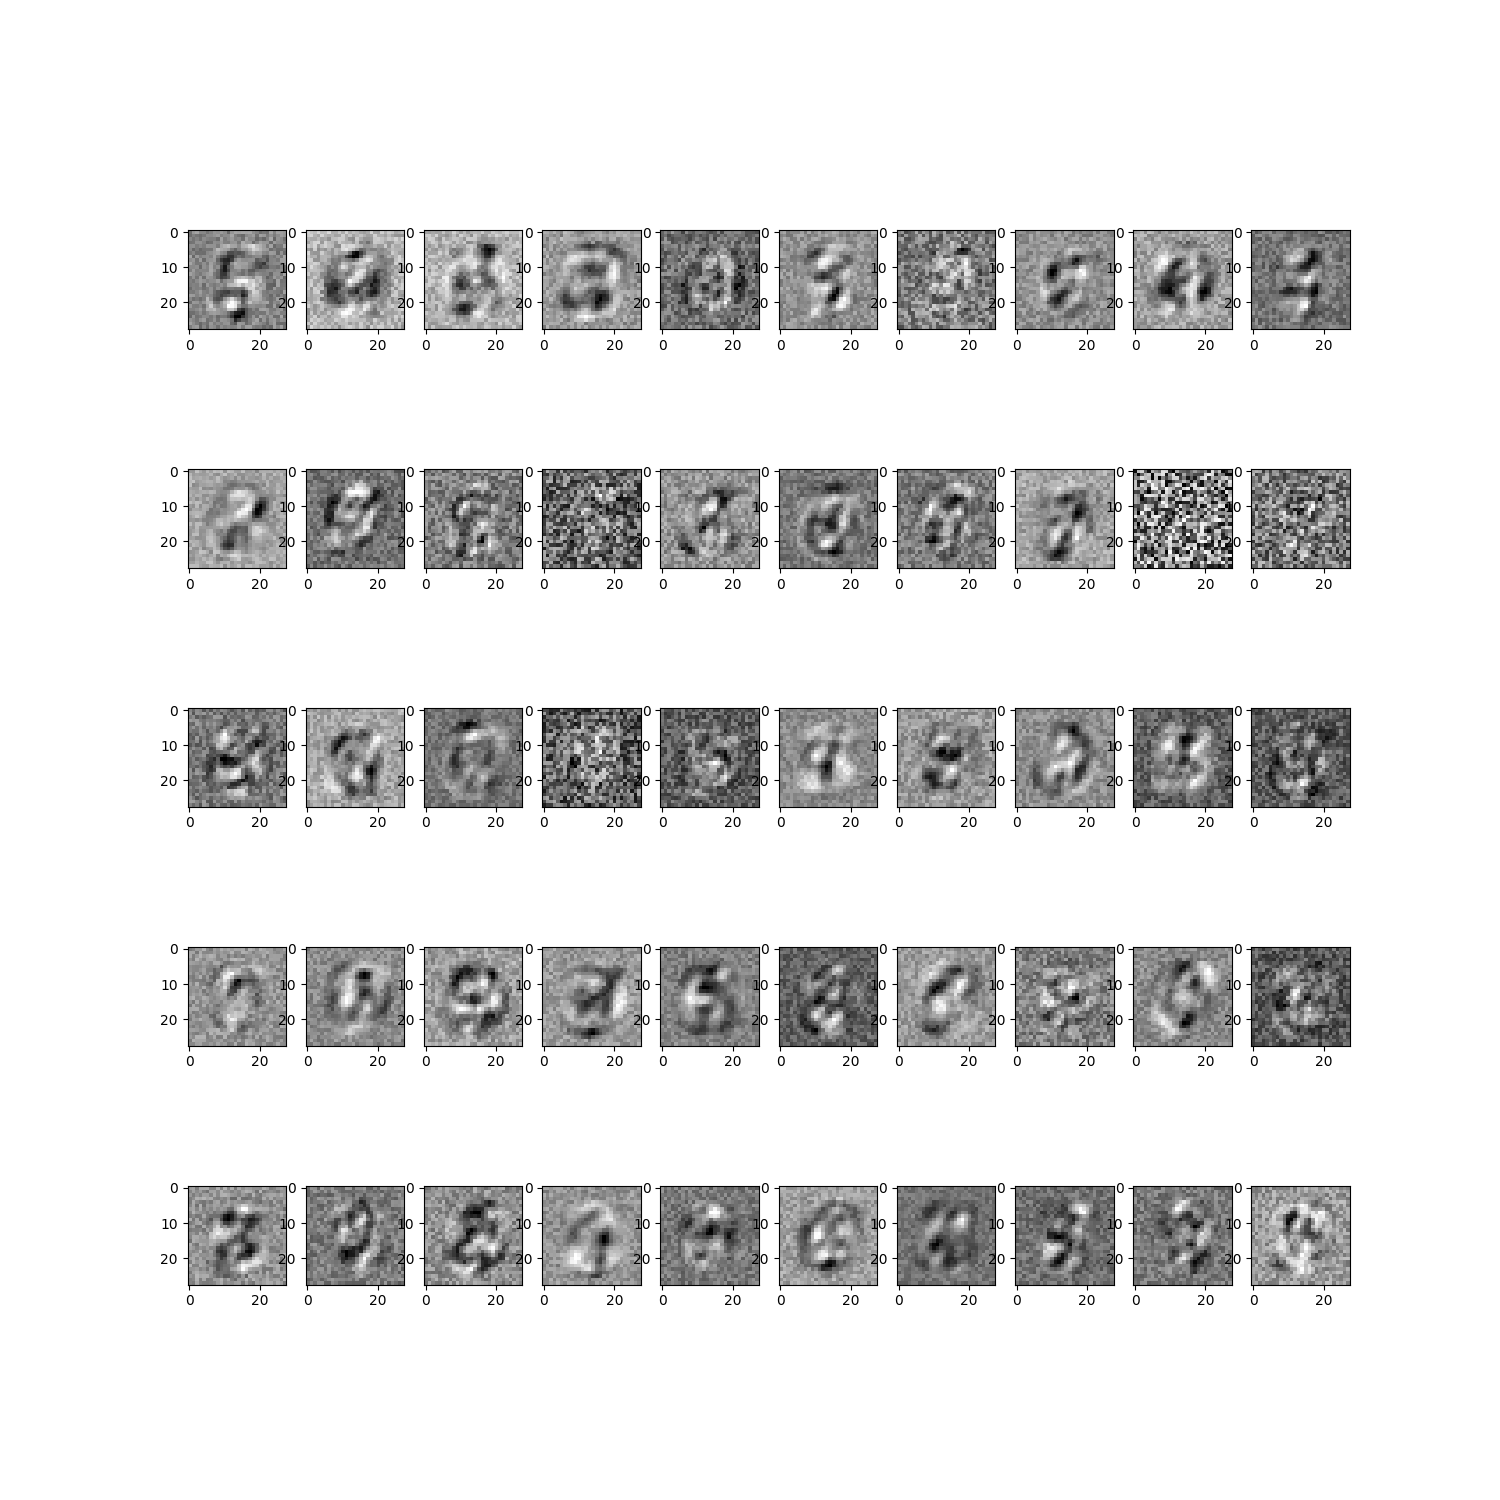
\includegraphics[width=0.9\textwidth]{../plots/3_1_2/last_layer_50_components_100e.png}
    \caption{AE weights, 50 hidden units.}
  \end{subfigure}
  ~
  \begin{subfigure}[t]{0.47\textwidth}
    \centering
    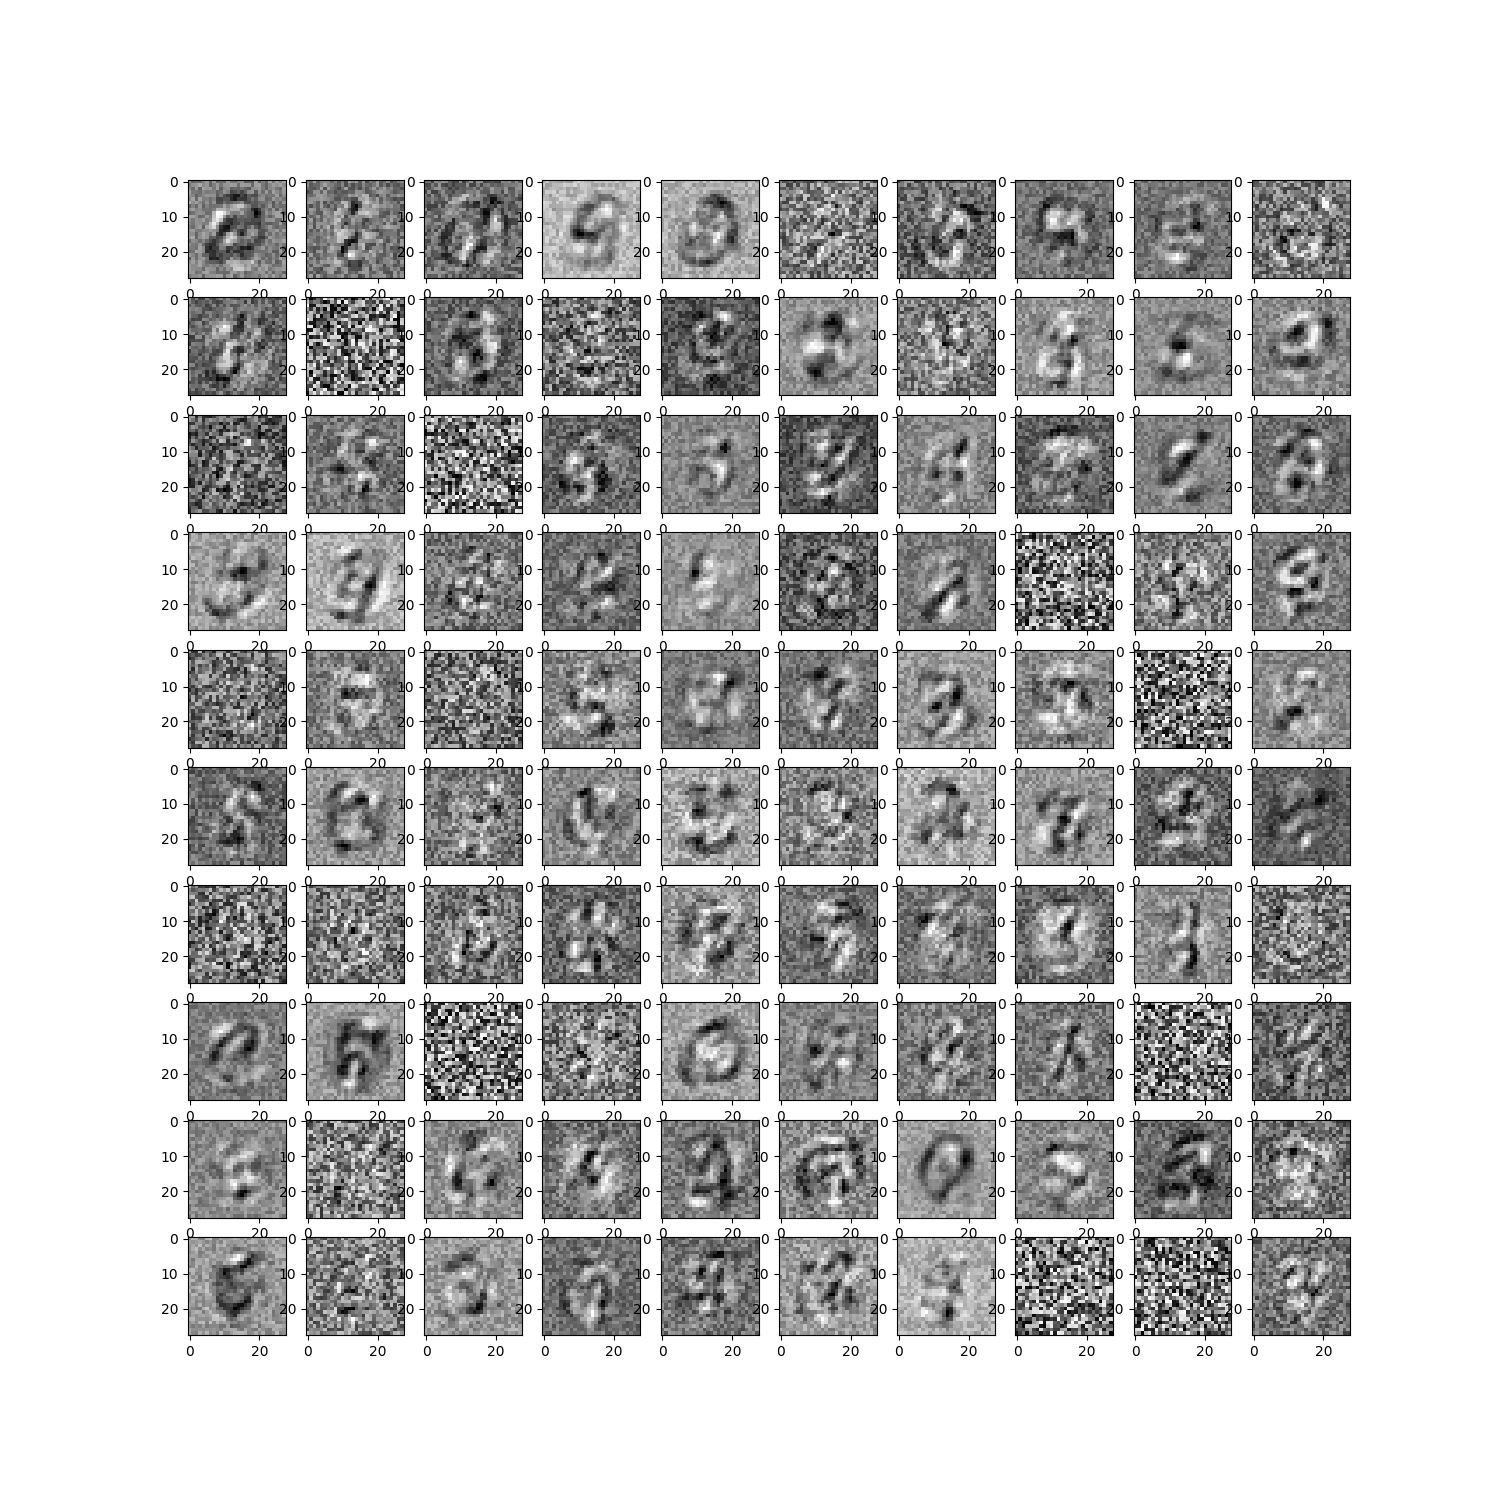
\includegraphics[width=0.9\textwidth]{../plots/3_1_2/last_layer_100_components_100e.png}
    \caption{AE weights, 100 hidden units.}
  \end{subfigure}
\end{figure}

\end{document}

